% **************************************************************************************************************
% A Classic Thesis Style
% An Homage to The Elements of Typographic Style
%
% Copyright (C) 2010 Andr� Miede http://www.miede.de
%
% If you like the style then I would appreciate a postcard. My address 
% can be found in the file ClassicThesis.pdf. A collection of the 
% postcards I received so far is available online at 
% http://postcards.miede.de
%
% License:
% This program is free software; you can redistribute it and/or modify
% it under the terms of the GNU General Public License as published by
% the Free Software Foundation; either version 2 of the License, or
% (at your option) any later version.
%
% This program is distributed in the hope that it will be useful,
% but WITHOUT ANY WARRANTY; without even the implied warranty of
% MERCHANTABILITY or FITNESS FOR A PARTICULAR PURPOSE.  See the
% GNU General Public License for more details.
%
% You should have received a copy of the GNU General Public License
% along with this program; see the file COPYING.  If not, write to
% the Free Software Foundation, Inc., 59 Temple Place - Suite 330,
% Boston, MA 02111-1307, USA.
%
% **************************************************************************************************************
% Note:
%    * You must not use "u etc. in strings/commands that will be spaced out (use \"u or real umlauts instead)
%    * New enumeration (small caps): \begin{aenumerate} \end{aenumerate}
%    * For margin notes: \graffito{}
%    * Do not use bold fonts in this style, it is designed around them
%    * Use tables as in the examples
%    * See classicthesis-ldpkg.sty for useful commands
% **************************************************************************************************************
% To Do:
%		 * [high] Check this out: http://www.golatex.de/koma-script-warnung-in-verbindung-mit-listings-package-t2058.html
%    * [medium] mathbb in section-titles/chapter-titles => disappears somehow in headlines!!!
%    * [low] Calculate text block size for Libertine font
%    * [low] Think about processing a4paper, a5paper, 10pt, 11pt, 12pt etc. options for typearea layout
%            (store values in internal variables and handle by \AtEndOfPackage{\areaset...})
% **************************************************************************************************************
\documentclass[ oneside,openright,titlepage,fleqn,numbers=noenddot,headinclude,%1headlines,% 
                11pt,a4paper,BCOR5mm,footinclude,cleardoublepage=empty,abstractoff,dottedtoc % <--- obsolete, remove (todo)
                ]{scrreprt}

% ********************************************************************
% Development Stuff
% ********************************************************************
\listfiles
%\usepackage[l2tabu, orthodox, abort]{nag}
%\usepackage[warning, all]{onlyamsmath}
% ********************************************************************
% Re-usable information
% ********************************************************************
\newcommand{\myTitle}{A Classic Thesis Style\xspace}
\newcommand{\myDegree}{An Homage to The Elements of Typographic Style\xspace}
\newcommand{\myName}{Andr\'e Miede\xspace}
\newcommand{\myProf}{Put name here\xspace}
\newcommand{\myOtherProf}{Put name here\xspace}
\newcommand{\mySupervisor}{Put name here\xspace}
\newcommand{\myFaculty}{Put data here\xspace}
\newcommand{\myDepartment}{Put data here\xspace}
\newcommand{\myUni}{\protect{Put data here}\xspace}
\newcommand{\myLocation}{Darmstadt\xspace}
\newcommand{\myTime}{May 2010\xspace}
\newcommand{\myVersion}{Version 2.8\xspace}
%*******************************************************
% Packages with options that might require adjustments
%*******************************************************
\usepackage[latin1]{inputenc} 
\usepackage[ngerman,american]{babel}           
% Maxnames gibt an wie viele Autoren ausgeschrieben werden.
% BibliographyStrings setzt den zu verwendenten Verkuerzungsstrings bei ueberschreiten (hier: et al.)
\usepackage[natbib=true,style=authoryear,maxnames=2]{biblatex}
\DefineBibliographyStrings{ngerman}{andothers={et \addabbrvspace al\adddot}}

% TODO: Pfad zur BibLaTeX Datei anpassen.
\bibliography{Bibliography}
\usepackage[fleqn]{amsmath} % math environments and more by the AMS 

%*******************************************************
\usepackage{classicthesis-ldpkg} % [backref]
%*******************************************************
% Options for classicthesis.sty:
% tocaligned eulerchapternumbers drafting linedheaders listsseparated 
% subfig nochapters beramono eulermath parts minionpro pdfspacing 
% listings dottedtoc minionprospacing manychapters
\usepackage[eulerchapternumbers,drafting,listings,listsseparated,%pdfspacing,%listings,
						subfig,beramono,eulermath,parts]{classicthesis}

%*******************************************************
% Some font experiments
%*******************************************************
%\usepackage[osf]{libertine}
%\usepackage{hfoldsty}
%\usepackage[light,condensed,math]{iwona}
%\renewcommand{\sfdefault}{iwona}
%\usepackage{lmodern} % <-- no osf support :-(
%\usepackage[urw-garamond]{mathdesign} <-- no osf support :-(

%*******************************************************
% Fine-tuning for the text area
%*******************************************************
%\linespread{1.05} % a bit more for Palatino
%\areaset[5mm]{312pt}{761pt} % 686 (factor 2.2) + 33 head + 42 head \the\footskip
%\setlength{\marginparwidth}{7em}%
%\setlength{\marginparsep}{2em}%

%*******************************************************
% hack to use citations in float environments 
% will be fixed with caption package version 3.2
%*******************************************************
\usepackage{makerobust} 
\makeatletter 
\MakeRobustCommand\caption@xref 
\makeatother 

%*******************************************************            
%\usepackage[section,below]{placeins} <--- not everybody wants this
%\usepackage[all]{hypcap} <--- does not work with MiKTeX 2.6
% ********************************************************************
% Language/strings for backrefs (change here, thanks, Lorenzo)
%*******************************************************
%\renewcommand{\backrefnotcitedstring}{\relax}%(Not cited.)
%\renewcommand{\backrefcitedsinglestring}[1]{(Citato a pagina~#1.)}
%\renewcommand{\backrefcitedmultistring}[1]{(Citato alle pagine~#1.)}
%\renewcommand{\backreftwosep}{ e~}
%\renewcommand{\backreflastsep}{ e~}
% ********************************************************************
% Setup and Finetuning
%*******************************************************
\newlength{\abcd} % for ab..z string length calculation
\newcommand{\myfloatalign}{\centering} % how all the floats will be aligned
\setlength{\extrarowheight}{3pt} % increase table row height
% ********************************************************************
% Captions look and feel
%*******************************************************
\captionsetup{format=hang,font=small}
% ********************************************************************
% Listings setup
% ********************************************************************
%\lstset{emph={trueIndex,root},emphstyle=\color{BlueViolet}}%\underbar} % for special keywords
% ********************************************************************
\lstset{%C++,
    keywordstyle=\color{RoyalBlue},%\bfseries,
    basicstyle=\small\ttfamily,
    %identifierstyle=\color{NavyBlue},
    commentstyle=\color{Green}\ttfamily,
    stringstyle=\rmfamily,
    numbers=none,%left,%
    numberstyle=\scriptsize,%\tiny
    stepnumber=5,
    numbersep=8pt,
    showstringspaces=false,
    breaklines=true,
    frameround=ftff,
    frame=single,
    belowcaptionskip=.75\baselineskip,
    numberbychapter=false
    %frame=L
} 

% ********************************************************************
% Where to look for graphics
%*******************************************************
%\graphicspath{{gfx/}{misc/}} % considered harmful according to l2tabu
% ********************************************************************
% Hyperreferences
%*******************************************************
\hypersetup{%
    colorlinks=true, linktocpage=true, pdfstartpage=3, pdfstartview=FitV,%
    % uncomment the following line if you want to have black links (e.g., for printing)
    %colorlinks=false, linktocpage=false, pdfborder={0 0 0}, pdfstartpage=3, pdfstartview=FitV,% 
    breaklinks=true, pdfpagemode=UseNone, pageanchor=true, pdfpagemode=UseOutlines,%
    plainpages=false, bookmarksnumbered, bookmarksopen=true, bookmarksopenlevel=1,%
    hypertexnames=true, pdfhighlight=/O,%hyperfootnotes=true,%nesting=true,%frenchlinks,%
    urlcolor=webbrown, linkcolor=RoyalBlue, citecolor=webgreen, %pagecolor=RoyalBlue,%
    %urlcolor=Black, linkcolor=Black, citecolor=Black, %pagecolor=Black,%
    pdftitle={\myTitle},%
    pdfauthor={\textcopyright\ \myName, \myUni, \myFaculty},%
    pdfsubject={},%
    pdfkeywords={},%
    pdfcreator={pdfLaTeX},%
    pdfproducer={LaTeX with hyperref and classicthesis}%
}

%********************************************************************
% Hyphenation
%*******************************************************
%\hyphenation{put special hyphenation here}
% ********************************************************************
% GO!GO!GO! MOVE IT!
%*******************************************************
\begin{document}
\frenchspacing
\raggedbottom
\selectlanguage{american} % american ngerman
%\renewcommand*{\bibname}{new name}
%\setbibpreamble{}
\pagenumbering{roman}
\pagestyle{plain}
%********************************************************************
% Frontmatter
%*******************************************************
%*******************************************************
% Titlepage
%*******************************************************
\begin{titlepage}
	% if you want the titlepage to be centered, uncomment and fine-tune the line below (KOMA classes environment)
	\begin{addmargin}[-1cm]{-3cm}
    \begin{center}
        \large  

        \hfill

        \vfill

        \begingroup
            \color{Maroon}\spacedallcaps{\myTitle} \\ \bigskip
        \endgroup

        \spacedlowsmallcaps{\myName}
        
        \spacedlowsmallcaps{\myPersonId}

        \vfill

        % 
\includegraphics[width=6cm]{gfx/TFZsuperellipse_bw} \\ \medskip

        \myDegree \\ \medskip   
        %\myDepartment \\                            
        %\myFaculty \\
        %\myUni \\ \bigskip

        \myTime

        \vfill                      

    \end{center}  
  \end{addmargin}       
\end{titlepage}   
\pagestyle{scrheadings}
\cleardoublepage%*******************************************************
% Table of Contents
%*******************************************************
%\phantomsection
\refstepcounter{dummy}
\pdfbookmark[1]{\contentsname}{tableofcontents}
\setcounter{tocdepth}{2} % <-- 2 includes up to subsections in the ToC
\setcounter{secnumdepth}{3} % <-- 3 numbers up to subsubsections
\manualmark
\markboth{\spacedlowsmallcaps{\contentsname}}{\spacedlowsmallcaps{\contentsname}}
\tableofcontents 
\automark[section]{chapter}
\renewcommand{\chaptermark}[1]{\markboth{\spacedlowsmallcaps{#1}}{\spacedlowsmallcaps{#1}}}
\renewcommand{\sectionmark}[1]{\markright{\thesection\enspace\spacedlowsmallcaps{#1}}}%*******************************************************
% List of Figures and of the Tables
%*******************************************************
\clearpage

\begingroup 
    \let\clearpage\relax
    \let\cleardoublepage\relax
    \let\cleardoublepage\relax
    %*******************************************************
    % List of Figures
    %*******************************************************    
    %\phantomsection 
    \refstepcounter{dummy}
    %\addcontentsline{toc}{chapter}{\listfigurename}
    \pdfbookmark[1]{\listfigurename}{lof}
    \listoffigures

    \vspace*{8ex}

    %*******************************************************
    % List of Tables
    %*******************************************************
    %\phantomsection 
    \refstepcounter{dummy}
    %\addcontentsline{toc}{chapter}{\listtablename}
    \pdfbookmark[1]{\listtablename}{lot}
    \listoftables
        
    \vspace*{8ex}
%   \newpage
    
    %*******************************************************
    % List of Listings
    %*******************************************************      
	  %\phantomsection 
    \refstepcounter{dummy}
    %\addcontentsline{toc}{chapter}{\lstlistlistingname}
    \pdfbookmark[1]{\lstlistlistingname}{lol}
    \lstlistoflistings 

    \vspace*{8ex}
       
    %*******************************************************
    % Acronyms
    %*******************************************************
    %\phantomsection 
    \refstepcounter{dummy}
    \pdfbookmark[1]{Acronyms}{acronyms}
    \markboth{\spacedlowsmallcaps{Acronyms}}{\spacedlowsmallcaps{Acronyms}}
    \chapter*{Acronyms}
    \begin{acronym}[UML]
    	\acro{AR}{Additional-Requirements}
    	\acro{FR}{Favourite-Requirements}
		\acro{GR}{GUI-Requirements}    	
    	\acro{GUI}{graphical user interface}
    	\acro{HPR}{Homepage-Requirements}
        \acro{HR}{History-Requirements}
        \acro{HTML}{HyperText Markup Language}
        \acro{HTTP}{Hypertext Transfer Protocol}
        \acro{PR}{Printing-Requirements}
        \acro{URL}{Uniform Resource Locator}
        \acro{WR}{Web-Requirements}
    \end{acronym}                     
\endgroup

\cleardoublepage
%********************************************************************
% Mainmatter
%*******************************************************
\pagenumbering{arabic}
% use \cleardoublepage here to avoid problems with pdfbookmark
\cleardoublepage\part{Development of StockCess}
%************************************************
\chapter{Introduction}\label{ch:introduction}
%************************************************

In this chapter an overview over the document, as well as the specified requirements shall be given.

\section{Document overview}
\label{sec:document_overview}

This report fulfils in major parts the role of a requirements document. As such, it is intended for different audiences:
\autoref{ch:requirements} provides an overview over the fulfilled requirements and thus should be of greatest interest for the managerial department, as well as the end users.

\autoref{ch:user_guide} is a user guide that showcases the use of the program by showing how to accomplish certain tasks with the application. This part is essential for end users.

\autoref{ch:design} and \autoref{ch:developer_guide} are intended for engineers and software developers. They provide an overview over the application's high- and low-level design, highlighting certain important aspects that might need to be taken into account to allow further development to proceed at an efficient pace.

\autoref{ch:testing} provides an overview over the testing that has happened during the development.

\autoref{ch:conclusions} will wrap up the development of the application and provide an outlook at possible improvements that might be made.

\section{Remit}
\label{sec:remit}

This section shall provide a short recap of the specified requirements. A list of fulfilled requirements will be provided in \autoref{ch:requirements}.

The requirements, as understood by the contractor, are as follows \footnote{For further reference the requirements are prefixed with unique numbers: \ac{MSI}, \ac{MBA}, \ac{MDA}, \ac{GUI}}:

\begin{description}
\item[MSI01:] Allow the management of \textit{stock items}. Management includes the following operations: \textit{add}, \textit{edit}, \textit{delete}.
\item[MSI02:] The operation \textit{add} and \textit{delete} should be possible without the use of an external storage.
\item[MSI03:] Every stock item should consist of the following attributes: a \textit{Stock Code}, an \textit{item name}, a \textit{supplier name}, a \textit{unit's cost}, the \textit{number required} and the \textit{current stock}\footnote{For verification purposes it was assumed that the stock code is 4-digit number with trailing zeros allowed.}.
\item[MSI04:] Allow the ordering of stock items via a money transfer.
\item[MBA01:] Allow the management of \textit{bank accounts}: Management includes the following operations: \textit{add}, \textit{edit}, \textit{delete}.
\item[MBA02:] The real transaction of money needs \textbf{not} to be implemented.
\item[MBA03:] An order should deduct the needed money from the bank account and change the \textit{required} and \textit{current} stock of an item accordingly.
\item[MDA01:] Allow the import and export of \textit{stock items} from \ac{CSV}-file.
\item[MDA02:] The location of the file may be chosen by the user.
\item[MDA03:] The ordering of the \ac{CSV}-file may not be changed.
\item[MDA04:] The ordering of the file is as follows:
\begin{lstlisting}
StockCode,Name,SupplierName,UnitCost,RequiredStock,CurrentStock
\end{lstlisting}
\item[MDA04:] The file should support blank fields by not entering data between two commas.
\item[MDA05:] The application should be able to handle \textit{at least} 100 items.
\item[GUI01:] Interaction between user and program shall happen via a \ac{GUI}.
\item[GUI02:] The \ac{GUI} shall provide menus, buttons and icons for easier accessibility.
\end{description}

%************************************************
\chapter{Requirement's checklist}\label{ch:requirements} % $\mathbb{ZNR}$
%************************************************

The following list shall provide an overview over the fulfilled requirements.
The numbers correspond to those used in \autoref{ch:introduction}.

\begin{description}
\item[HO01:] Fulfilled.
\item[HO02:] Fulfilled.
\item[HO03:] Fulfilled.
\item[HO04:] Fulfilled.
\item[SE01:] Fulfilled.
\item[SE02:] Fulfilled.
\item[SE03:] Fulfilled.
\item[PR01:] Fulfilled.
\item[PR02:] Fulfilled.
\item[PR03:] Fulfilled.
\item[PR04:] Fulfilled.
\item[SHO01:] Fulfilled.
\item[SHO02:] Partially - to guarantee the best user experience adding items is only supported from the search.
\item[SHO03:] Fulfilled.
\item[SHO04:] Fulfilled.
\item[SHO05:] Fulfilled.
\end{description}

Apart from these requirements the following features have been added to the application to enhance the user-experience:

\begin{description}
\item[Register as new user:] New users are provided with the option to set up a new user account to use the site.
\item[Error Notification:] Upon entering invalid information the user will be informed about the mistakes.
\end{description}
%\addtocontents{toc}{\protect\clearpage} % <--- just debug stuff, ignore
%************************************************
\chapter{Design considerations}\label{ch:design} % $\mathbb{ZNR}$
%************************************************


%************************************************
\chapter{User Guide}\label{ch:user_guide} % $\mathbb{ZNR}$
%************************************************

In this chapter ways to achieve the most common use-cases of the program will be explained. These include:

\begin{enumerate}
\item Managing (adding, deleting, editing) a stock item or bank account.
\item Placing an order.
\item Importing and exporting data.
\end{enumerate}

\section{Manage stock items and bank accounts}
\label{sec:manage_stock_item}

Upon starting the application the main window will be displayed.
The main window hosts all necessary controls for the first two use cases.

\begin{figure}[H]
\begin{center}
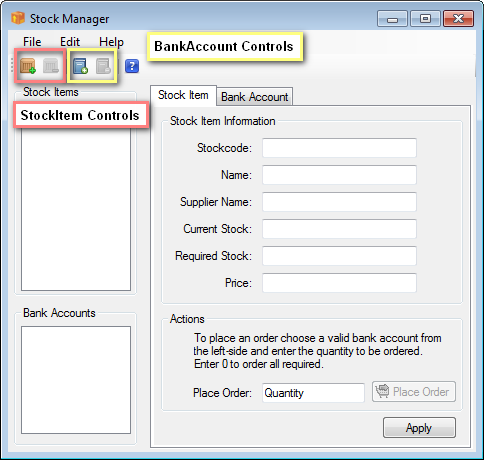
\includegraphics[width=0.8\textwidth]{gfx/main_window.png}
\caption{Main Window}
\label{fig:main_window}
\end{center}
\end{figure}

To add a stock item or a bank account a click on the appropriate button is necessary:
 
% content section
\begin{wrapfigure}{l}{5cm} % "l" or "r" for the side on the page. And the width parameter for the width of the image space.
\centering

\includegraphics[scale=1]{gfx/add_stock_item.png}
\caption{Add a stock item.}
\label{fig:add_si}
\end{wrapfigure}

By clicking the icon to add a new stock item to the application, an item will be inserted into the stock item list with dummy values.

\begin{wrapfigure}{l}{5cm} % "l" or "r" for the side on the page. And the width parameter for the width of the image space.
\centering

\includegraphics[scale=1]{gfx/add_bank_account.png}
\caption{Add a bank account.}
\label{fig:add_ba}
\end{wrapfigure}

By clicking the icon to add a new bank account to the application, a account will be inserted into the bank account list with dummy values.

After inserting a new stock item or bank account, the item can be chosen in the appropriate list (on the left-hand side of the application). By clicking an item, the appropriate panel will be show up, where the values can be edited.

Editing needs to be completed by clicking the \textit{apply}-button. If any incorrect values were entered, the application will inform the user about the occured mistakes.

To manage a bank account there are two more possible commands the user can issue: apart from changing the values, it is possible to deposit or withdraw money from the bank account. Therefore the user simply has to enter a number in the correct field and press the accompanying button.

\begin{figure}[H]
\begin{center}
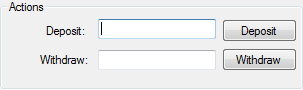
\includegraphics[scale=1.0]{gfx/bank_account_actions.png}
\caption{Depositing and withdrawing money}
\label{fig:ba_actions}
\end{center}
\end{figure}

\section{Placing an order}
\label{sec:placing_order}

\begin{wrapfigure}[11]{l}{5cm} % "l" or "r" for the side on the page. And the width parameter for the width of the image space.
\centering
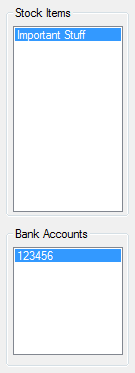
\includegraphics[scale=0.6]{gfx/highlighted_items.png}
\caption{Selection of items.}
\label{fig:highlighted_items}
\end{wrapfigure}

To place an order the user has to select a bank account and a stock item from the lists (an item needs to be highlighted in both lists).

Then a value can be entered inside the \textit{quantity}-box: either the amount of items to be ordered, or 0. By entering 0 the program will try to order the \textit{required amount}.

If enough funds are available the order will be placed and the stock information will be updated.
If not enough funds are available the application will output an error message.

\begin{figure}[H]
\begin{center}
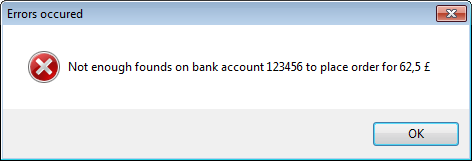
\includegraphics[scale=0.8]{gfx/not_enough_funds.png}
\caption{Placing an order without the needed funds}
\label{fig:not_enough_funds}
\end{center}
\end{figure}


\section{Importing \& exporting data}
\label{sec:import_export}

After entering stock items and bank accounts it is possible to save them to a file and open them again for later use.

Therefore the user has to choose the appropriate option from the file menu or set standard-paths and click the menu-bar icon.

\subsection{File menu}
\label{subsec:file_menu}

To save or load only one of the list the user selects \texttt{File $\Rightarrow$ Save (Open) $\Rightarrow$ Save (Open) bank accounts / Save (Open) stock items}.

\begin{figure}[H]
\begin{center}
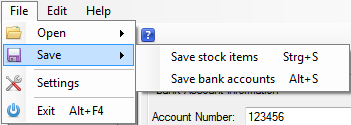
\includegraphics[scale=0.8]{gfx/save_file_menu.png}
\caption{Saving via file menu}
\label{fig:save_file_menu}
\end{center}
\end{figure}

\subsection{Menu-bar icon}

To save via the menu icon it is necessary to first set default file paths for the files \footnote{As soon as these paths are set, the application will also attempt to load items and bank account on start-up.}. The paths can be set in the \texttt{settings window} found under \texttt{File $\Rightarrow$ Settings}.

\begin{figure}[H]
\begin{center}
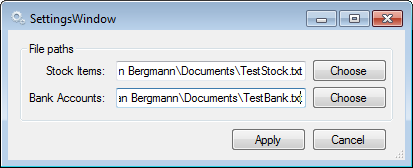
\includegraphics[scale=0.8]{gfx/settings_window.png}
\caption{Settings window}
\label{fig:settings_window}
\end{center}
\end{figure}

After setting these paths both lists can be saved with a single click on the menu-bar icon (denoted by two disks).

%************************************************
\chapter{Developer Guide}\label{ch:developer_guide} % $\mathbb{ZNR}$
%************************************************
%************************************************
\chapter{Testing}\label{ch:testing} % $\mathbb{ZNR}$
%************************************************

The testing of the application was performed in two stages:

\begin{itemize}
\item In the early development stages unit-tests were written for the base classes.
\item After chaining the application parts together, the applications correct behaviour was mainly tested by using the application. This was necessary as unit-testing \ac{GUI} and multi-threaded code is extremely difficult.
\end{itemize}

\section{Unit-tests}
\label{sec:unit_tests}

The source-code of the written unit-tests can be seen in \autoref{ap:tests}.

To run the test-cases the \href{http://www.nunit.org/}{NUnit}-framework (\url{http://www.nunit.org/}) is needed.

The test-cases cover the passing of different types of parameters.

A short list shall be provided:



\section{Acceptance-tests}
\label{sec:acceptance_tests}

%************************************************
\chapter{Conclusions}\label{ch:conclusions} % $\mathbb{ZNR}$
%************************************************
%\include{multiToC} % <--- just debug stuff, ignore for your documents
% ********************************************************************
% Backmatter
%*******************************************************
\appendix
\cleardoublepage\part{Appendix}
%********************************************************************
% Appendix
%*******************************************************
\chapter{Appendix: Source Code}
\label{appendix}

\section{GUI}
\label{ap:gui}

\sourcePackage{Assessment_Two}{GUI}

\sourceClass{ThreadingView.cs}

\sourceClass{MainWindow.cs}

\sourceClass{FavouriteWindow.cs}

\sourceClass{SettingsWindow.cs}

\section{Logic}
\label{ap:logic}

\subsection{Interfaces}

\sourcePackage{Assessment_Two_Logic/Interfaces}{Interfaces}

\sourceClass{IFavouritesView.cs}
\sourceClass{IFavouriteView.cs}
\sourceClass{IHistoryView.cs}
\sourceClass{IPrintView.cs}
\sourceClass{ISerialiser.cs}
\sourceClass{IView.cs}
\sourceClass{IWebPageView.cs}

\subsection{Model}

\sourcePackage{Assessment_Two_Logic/Model}{Model}

\sourceClass{ErrorMessage.cs}
\sourceClass{ErrorMessageCollection.cs}
\sourceClass{Favourite.cs}
\sourceClass{FavouriteHandler.cs}
\sourceClass{History.cs}
\sourceClass{HistoryHandler.cs}
\sourceClass{NoFilePathSetException.cs}
\sourceClass{PageHandler.cs}
\sourceClass{SerializableDictionary.cs}
\sourceClass{SimpleWebResponse.cs}
\sourceClass{XmlSerialiser.cs}

\subsection{Presenter}

\sourcePackage{Assessment_Two_Logic/Presenter}{Presenter}

\sourceClass{FavouritePresenter.cs}
\sourceClass{FavouritesPresenter.cs}
\sourceClass{HistoryPresenter.cs}
\sourceClass{PagePresenter.cs}
\sourceClass{PrintPresenter.cs}

\section{Tests}
\label{ap:tests}
%********************************************************************
% Other Stuff in the Back
%*******************************************************
\cleardoublepage%********************************************************************
% Bibliography
%*******************************************************
% work-around to have small caps also here in the headline
\manualmark
\markboth{\spacedlowsmallcaps{\bibname}}{\spacedlowsmallcaps{\bibname}} % work-around to have small caps also
%\phantomsection 
\refstepcounter{dummy}
\addtocontents{toc}{\protect\vspace{\beforebibskip}} % to have the bib a bit from the rest in the toc
\addcontentsline{toc}{chapter}{\tocEntry{\bibname}}
\printbibliography{}
\label{app:bibliography} 
% \cleardoublepage\pagestyle{empty}

\hfill

\vfill


\pdfbookmark[0]{Colophon}{colophon}
\section*{Colophon}
This thesis was typeset with \LaTeXe\ using Hermann Zapf's
\emph{Palatino}
and \emph{Euler} type faces (Type~1 PostScript fonts \emph{URW
Palladio L}
and \emph{FPL} were used). The listings are typeset in \emph{Bera
Mono}, originally developed by Bitstream, Inc. as ``Bitstream Vera''.
(Type~1 PostScript fonts were made available by Malte Rosenau and
Ulrich Dirr.)

The typographic style was inspired by \cauthor{bringhurst:2002}'s genius as
presented in \emph{The Elements of Typographic Style} 
\citep{bringhurst:2002}. It is available for \LaTeX\ via \textsmaller{CTAN} as 
``\href{http://www.ctan.org/tex-archive/macros/latex/contrib/classicthesis/}%
{\texttt{classicthesis}}''.

\paragraph{note:} The custom size of the textblock was calculated
using the directions given by Mr. Bringhurst (pages 26--29 and
175/176). 10~pt Palatino needs  133.21~pt for the string
``abcdefghijklmnopqrstuvwxyz''. This yields a good line length between
24--26~pc (288--312~pt). Using a ``\emph{double square textblock}''
with a 1:2 ratio this results in a textblock of 312:624~pt (which
includes the headline in this design). A good alternative would be the
``\emph{golden section textblock}'' with a ratio of 1:1.62, here
312:505.44~pt. For comparison, \texttt{DIV9} of the \texttt{typearea}
package results in a line length of 389~pt (32.4~pc), which is by far
too long. However, this information will only be of interest for
hardcore pseudo-typographers like me.%

To make your own calculations, use the following commands and look up
the corresponding lengths in the book:
\begin{verbatim}
    \settowidth{\abcd}{abcdefghijklmnopqrstuvwxyz}
    \the\abcd\ % prints the value of the length
\end{verbatim}
Please see the file \texttt{classicthesis.sty} for some precalculated 
values for Palatino and Minion.

    \settowidth{\abcd}{abcdefghijklmnopqrstuvwxyz}
    \the\abcd\ % prints the value of the length


\bigskip

\noindent\finalVersionString




% \cleardoublepage%*******************************************************
% Declaration
%*******************************************************
\refstepcounter{dummy}
\pdfbookmark[0]{Declaration}{declaration}
\chapter*{Declaration}
\thispagestyle{empty}
Put your declaration here.
\bigskip
 
\noindent\textit{\myLocation, \myTime}

\smallskip

\begin{flushright}
    \begin{tabular}{m{5cm}}
        \\ \hline
        \centering\myName \\
    \end{tabular}
\end{flushright}

% ********************************************************************
% Game Over: Restart, Restore or Quit?
%*******************************************************
\end{document}
% ********************************************************************
